\chapter{Verifica della Trasferibilità degli Attacchi}
    In questo capitolo analizziamo la trasferibilità degli adversarial attacks, ovvero la loro capacità di ingannare modelli differenti da quello bersaglio utilizzato per la generazione. Questa proprietà è particolarmente pericolosa in ambito di sicurezza, poiché consente a un attaccante di compromettere un sistema anche senza conoscere la sua architettura interna, basandosi solo su un modello sostitutivo.
    Per valutare la trasferibilità, abbiamo introdotto un secondo classificatore, denominato \textbf{NN2}, basato sull’architettura \textit{ResNet50}, pre-addestrato sul dataset VGG-Face2. Il modello è stato caricato con pesi ottimizzati (fine-tuning) corrispondenti a 8631 identità. La rete NN2 differisce in modo sostanziale da NN1 (modello usato per generare gli attacchi), offrendo quindi un contesto adatto per una valutazione realistica della robustezza cross-architettura.

    \section{Trasferibilità: Aspetti Teorici}
        La trasferibilità degli attacchi adversarial rappresenta uno dei fenomeni più rilevanti e preoccupanti nel contesto della sicurezza dei modelli di deep learning. Studi empirici e teorici hanno mostrato che input modificati per ingannare un determinato modello possono spesso mantenere la loro efficacia anche su modelli con architetture diverse o parametri differenti. Questo comportamento, noto come \textit{cross-model transferability}, si manifesta con particolare evidenza nei cosiddetti attacchi \textit{error-generic}, che mirano a ottenere una classificazione errata, indipendentemente dalla classe di destinazione.
        Il meccanismo alla base di questa proprietà è legato alla similarità strutturale tra le rappresentazioni interne apprese da modelli diversi, specialmente se addestrati sullo stesso dominio. Di conseguenza, le perturbazioni che alterano i confini decisionali in un modello possono avere un effetto simile anche su un altro. In contesti reali, ciò significa che un attaccante può generare un attacco utilizzando un modello accessibile (\textit{surrogate}) e poi utilizzarlo con successo contro un sistema chiuso o sconosciuto, senza la necessità di conoscere la sua struttura o i suoi pesi.
        La probabilità di successo della trasferibilità dipende da diversi fattori, tra cui l’intensità della perturbazione, la somiglianza tra le architetture e il tipo di attacco utilizzato. Gli attacchi targeted, ad esempio, richiedono che l’input venga classificato come una specifica classe bersaglio e tendono quindi a trasferirsi meno efficacemente rispetto a quelli non mirati. Tuttavia, anche in questi casi sono stati osservati effetti non trascurabili, soprattutto con architetture con strutture latenti simili.
        Nel contesto del nostro progetto, la valutazione della trasferibilità consente di stimare l’efficacia reale degli attacchi generati su NN1 quando applicati a NN2, fornendo così una misura indiretta della pericolosità di tali perturbazioni in uno scenario di tipo black-box.
    
    \section{Implementazione del Modello NN2}
        Il modello NN2 è stato caricato utilizzando la libreria \texttt{torchvision} e i pesi pre-addestrati sono stati caricati da un file \texttt{resnet50\_ft\_weight.pkl}. Prima di passare i dati in input alla rete, è stato necessario replicare il preprocessing previsto per il training originale:
            \begin{itemize}
              \item Le immagini, originariamente normalizzate in $[-1, 1]$, sono state scalate nel range $[0, 255]$
              
              \item I canali RGB sono stati convertiti in BGR
              
              \item È stata sottratta la media per canale usata durante il fine-tuning (\texttt{mean\_bgr} = [91.4953, 103.8827, 131.0912])
              
              \item Le immagini sono state ridimensionate da $160 \times 160$ a $224 \times 224$ pixel, come richiesto da ResNet50
            \end{itemize}
    
    \section{Obiettivo dell’Analisi}
        L’obiettivo di questo capitolo è verificare se gli \textit{adversarial examples} generati su NN1 sono in grado di compromettere anche NN2. Questo viene valutato riproducendo le predizioni di NN2 sugli stessi campioni avversari (salvati da attacchi come FGSM, BIM, PGD, ecc.) e confrontando le etichette predette con quelle corrette.
        Per mantenere la coerenza tra le classi, è stata implementata una procedura di mappatura tra le etichette predette da NN2 e quelle usate durante la generazione su NN1. In fase di test, sono state mascherate le uscite della rete NN2 per considerare solo le classi presenti nel test set, in modo da evitare interferenze da identità non presenti.
        Nei paragrafi successivi vengono presentati i risultati sperimentali relativi alla trasferibilità di ciascun attacco error-generic e poi in seguito error-specific.

    \section{Trasferibilità dell'attacco FGSM Non-Targeted}
        L'attacco \textbf{FGSM non-targeted}, generato sulla rete NN1, è stato valutato per verificarne la \textit{trasferibilità} verso il classificatore NN2 (ResNet50). In questo caso, l’obiettivo delle perturbazioni non è forzare una classe specifica, ma semplicemente indurre una classificazione errata. L’efficacia della trasferibilità è stata misurata tramite l’accuratezza residua di NN2 nel classificare correttamente i campioni avversari.
        Il grafico in Figura~\ref{fig:fgsm_untargeted_transfer} mostra il comportamento dell'accuratezza del modello NN2 rispetto alla \textit{perturbazione media} introdotta, misurata in norma L$\infty$.
        
        \begin{figure}[H]
          \centering
          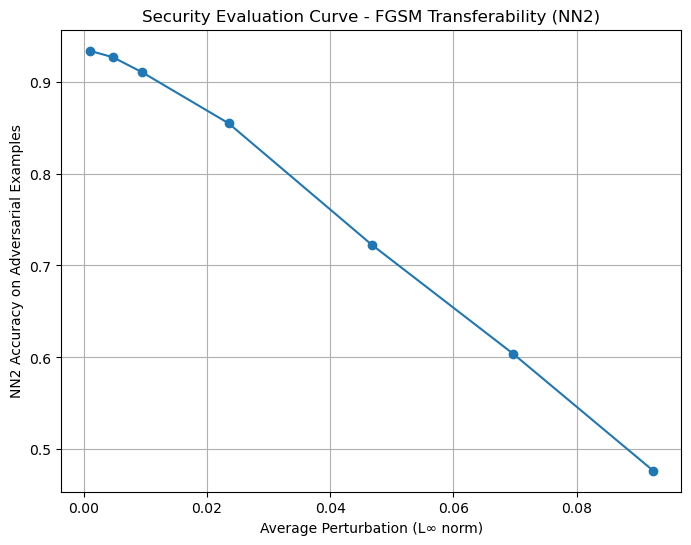
\includegraphics[width=0.7\textwidth]{images/untargFGSMtrasf.png}
          \caption{Security Evaluation Curve - FGSM Transferability (Non-Targeted, NN2)}
          \label{fig:fgsm_untargeted_transfer}
        \end{figure}

        \subsection{Osservazioni}
            I risultati numerici confermano un degrado progressivo delle prestazioni di NN2 all’aumentare della perturbazione:
                \begin{center}
                    \begin{tabular}{ccc}
                        \toprule
                        \textbf{Perturbazione media (L$_1$)} & \textbf{L$\infty$} & \textbf{Accuracy (\%)} \\
                        \midrule
                        0.0009 & 0.0010 & 93.36 \\
                        0.0047 & 0.0050 & 92.65 \\
                        0.0094 & 0.0100 & 91.03 \\
                        0.0235 & 0.0250 & 85.47 \\
                        0.0467 & 0.0500 & 72.26 \\
                        0.0697 & 0.0750 & 60.38 \\
                        0.0924 & 0.1000 & 47.67 \\
                        \bottomrule
                    \end{tabular}
                \end{center}

        \subsection{Analisi}
            L'attacco FGSM non-targeted mostra un'evidente capacità di trasferirsi da NN1 a NN2. Anche con perturbazioni di modesta entità (ad esempio L$\infty=0.025$), l'accuratezza del modello di destinazione si riduce significativamente. Con un'intensità massima (L$\infty=0.1$), la rete ResNet50 commette errori su oltre metà dei campioni avversari, dimostrando la vulnerabilità del sistema anche in uno scenario completamente black-box.
            Questo comportamento conferma quanto ampiamente documentato in letteratura, ovvero che gli attacchi \textit{non-targeted}, meno vincolati rispetto a quelli \textit{targeted}, tendono a produrre perturbazioni più generiche, in grado di colpire modelli con strutture interne differenti. La loro semplicità di generazione li rende strumenti particolarmente pericolosi in contesti in cui l’attaccante non ha accesso diretto al modello bersaglio.

    \section{Trasferibilità dell'attacco BIM Non-Targeted}
        L'attacco \textbf{Basic Iterative Method} (BIM), generato a partire dal modello NN1, è stato analizzato per verificarne la \textit{trasferibilità} verso NN2. A differenza di FGSM, BIM applica la perturbazione in modo iterativo, accumulando modifiche lungo la direzione del gradiente a ogni passo. Questo lo rende un attacco più preciso, ma potenzialmente anche più overfittato al modello di origine. L’obiettivo di questa analisi è determinare se tale maggiore precisione comprometta la capacità di trasferirsi verso architetture differenti.
        Nel grafico di Figura~\ref{fig:bim_transfer} è riportata la curva di accuratezza residua di NN2 rispetto alla perturbazione media, considerando tre configurazioni di attacco (5, 10 e 20 iterazioni) a parità di $\epsilon$ massimo.

        \begin{figure}[H]
          \centering
          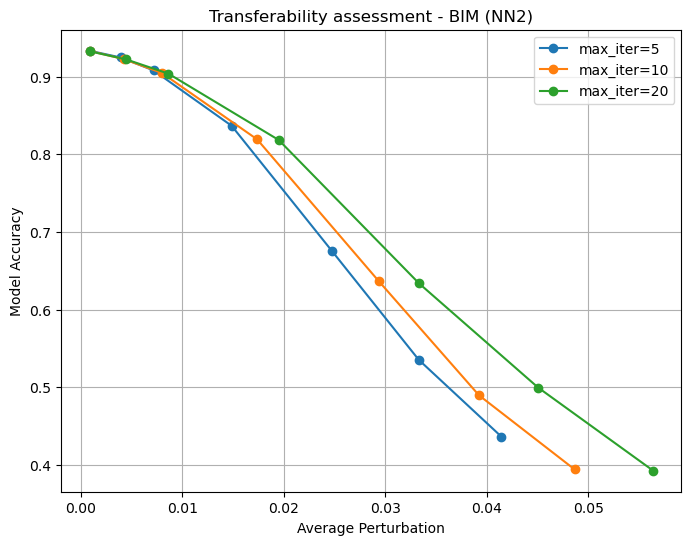
\includegraphics[width=0.7\textwidth]{images/untargBIMtrasf.png}
          \caption{Transferability assessment - BIM (NN2)}
          \label{fig:bim_transfer}
        \end{figure}

        \subsection{Osservazioni}
            La tabella seguente mostra i valori ottenuti per alcune delle principali configurazioni testate. Le perturbazioni sono espresse in norma L$\infty$ media, mentre l’accuratezza riflette la percentuale di predizioni corrette effettuate da NN2:
                \begin{center}
                    \begin{tabular}{cccc}
                        \toprule
                        \textbf{max\_iter} & \textbf{Perturbazione media} & \textbf{L$\infty$} & \textbf{Accuracy (\%)} \\
                        \midrule
                        5  & 0.0414 & 0.1000 & 43.65 \\
                        10 & 0.0487 & 0.1000 & 39.41 \\
                        20 & 0.0564 & 0.1000 & 39.24 \\
                        \bottomrule
                    \end{tabular}
                \end{center}

        \subsection{Analisi}
            I risultati mostrano che, come per FGSM, anche l’attacco BIM è in grado di trasferirsi da NN1 a NN2 in modo efficace. L’aumento del numero di iterazioni comporta una perturbazione media più ampia, ma la differenza di accuratezza residua tra $max\_iter = 10$ e $20$ è marginale, suggerendo una saturazione dell'effetto dopo un certo numero di passi.
            Con L$\infty = 0.1$ e perturbazioni medie comprese tra 0.04 e 0.056, l’accuratezza di NN2 scende sotto il 40\%, confermando la vulnerabilità cross-architettura del modello anche di fronte ad attacchi iterativi.
            Questi risultati indicano che, nonostante la maggiore specificità delle perturbazioni rispetto a FGSM, BIM mantiene un alto grado di trasferibilità, in particolare nelle configurazioni a media iterazione. Ciò lo rende una tecnica pericolosa anche in contesti black-box, dove l'attaccante può solo stimare la rete bersaglio.

    \section{Trasferibilità dell'attacco PGD Non-Targeted}
        L’attacco \textbf{Projected Gradient Descent} (PGD) rappresenta una generalizzazione iterativa del metodo FGSM, con proiezione dentro la $\epsilon$-ball. È considerato uno degli attacchi più robusti in letteratura ed è comunemente utilizzato come benchmark per la valutazione della resilienza dei modelli. In questo esperimento, sono state generate perturbazioni su NN1 e successivamente testate sulla rete NN2 per valutare la \textit{trasferibilità} cross-architettura.
        La Figura~\ref{fig:pgd_transfer} riporta l’accuratezza del modello NN2 rispetto alla \textit{perturbazione media} introdotta, per due configurazioni di attacco: \texttt{max\_iter=10} e \texttt{max\_iter=20}.
        
        \begin{figure}[H]
          \centering
          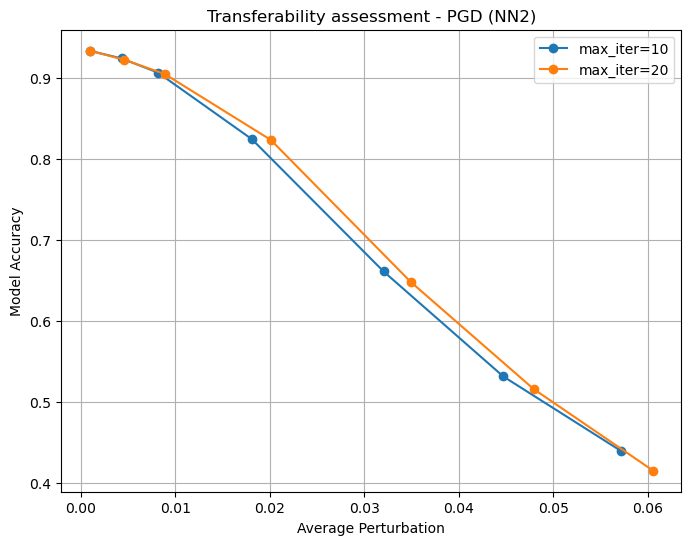
\includegraphics[width=0.7\textwidth]{images/untargPGDtrasf.png}
          \caption{Transferability assessment - PGD (NN2)}
          \label{fig:pgd_transfer}
        \end{figure}

        \subsection{Osservazioni}
            La tabella seguente riassume i risultati per i due setting di iterazioni. Come per BIM, è evidente un effetto di saturazione per iterazioni elevate, ma le prestazioni restano inferiori rispetto al test su immagini pulite:
                \begin{center}
                    \begin{tabular}{cccc}
                        \toprule
                        \textbf{max\_iter} & \textbf{Perturbazione media} & \textbf{L$\infty$} & \textbf{Accuracy (\%)} \\
                        \midrule
                        10 & 0.0009 & 0.0010 & 93.31 \\
                        10 & 0.0043 & 0.0050 & 92.36 \\
                        10 & 0.0082 & 0.0100 & 90.61 \\
                        10 & 0.0181 & 0.0250 & 82.39 \\
                        10 & 0.0320 & 0.0500 & 66.07 \\
                        10 & 0.0447 & 0.0750 & 53.11 \\
                        10 & 0.0571 & 0.1000 & 43.94 \\
                        \midrule
                        20 & 0.0010 & 0.0010 & 93.31 \\
                        20 & 0.0046 & 0.0050 & 92.19 \\
                        20 & 0.0089 & 0.0100 & 90.45 \\
                        20 & 0.0201 & 0.0250 & 82.31 \\
                        20 & 0.0349 & 0.0500 & 64.78 \\
                        20 & 0.0479 & 0.0750 & 51.58 \\
                        20 & 0.0606 & 0.1000 & 41.49 \\
                        \bottomrule
                    \end{tabular}
                \end{center}

        \subsection{Analisi}
            L’attacco PGD si dimostra altamente trasferibile verso NN2.
            Analizzando i dati nel dettaglio, si osserva che per $\epsilon \leq 0.005$, l’accuratezza di NN2 resta pressoché invariata sopra il 92\%, indipendentemente dal numero di iterazioni. In questo intervallo, l’effetto dell’attacco è minimo: la perturbazione media è troppo contenuta per produrre uno spostamento significativo nella distribuzione delle attivazioni interne.
            Superata la soglia di $\epsilon = 0.01$, l’impatto dell’attacco diventa più marcato: a $\epsilon = 0.025$, l’accuratezza scende all’82.39\% (con 10 iterazioni) e 82.31\% (con 20 iterazioni), mostrando una convergenza dei due setting e un iniziale effetto di saturazione. Ciò indica che il numero di iterazioni incide poco e che il limite dell'efficacia inizia a dipendere principalmente dal budget di perturbazione.
            Nella fascia intermedia ($\epsilon$ tra 0.05 e 0.075), l’effetto del numero di iterazioni inizia a emergere: si passa dal 66.07\% (iter=10) al 64.78\% (iter=20) e dal 53.11\% al 51.58\%, mostrando che iterazioni aggiuntive consentono una minima ma sistematica erosione delle performance del modello.
            A $\epsilon = 0.1$, entrambi i setting raggiungono il picco massimo di distorsione consentita, con perturbazioni medie pari a circa 0.057–0.060. L’accuratezza precipita rispettivamente al 43.94\% e 41.49\%, confermando che l’attacco è in grado di colpire la rete anche in profondità, inducendo errori sistematici. L’effetto di \texttt{max\_iter} tende a stabilizzarsi, segno che la strategia ha raggiunto la sua piena capacità d’impatto entro i 20 passi.
            Nel complesso, PGD dimostra un’ottima scalabilità e trasferibilità, con un comportamento coerente lungo tutta la curva e un degrado delle prestazioni che segue fedelmente l’intensità della perturbazione.
            Questi risultati consolidano PGD come una minaccia concreta anche in scenari black-box, grazie alla sua capacità di generare perturbazioni sufficientemente generiche da ingannare architetture differenti.

    \section{Trasferibilità dell'attacco DeepFool Non-Targeted}
        L'attacco \textbf{DeepFool} si basa su un approccio iterativo che mira a trovare la minima perturbazione possibile capace di condurre l'immagine oltre il confine decisionale del classificatore. A differenza degli altri metodi analizzati, DeepFool non impone vincoli espliciti sulla norma della perturbazione, ma ottimizza direttamente la distanza nel dominio delle decisioni. In questo esperimento, l’attacco è stato generato su NN1 e valutato su NN2 per stimare la capacità di trasferimento di perturbazioni minimali.
        Il test è stato condotto su un sottoinsieme di soli 10 campioni (a causa della complessità computazionale dell’attacco), selezionati in modo da garantire eterogeneità nelle classi di appartenenza.
        La Figura~\ref{fig:deepfool_transfer} mostra il singolo punto sperimentale ottenuto, rappresentante l’accuratezza di NN2 rispetto alla perturbazione media introdotta.
        
        \begin{figure}[H]
          \centering
          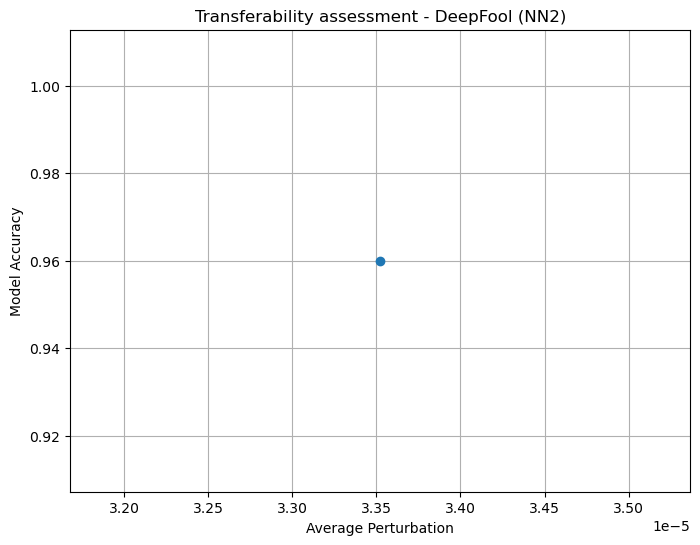
\includegraphics[width=0.65\textwidth]{images/untargDFtrasf.png}
          \caption{Transferability assessment - DeepFool (NN2).}
          \label{fig:deepfool_transfer}
        \end{figure}

        \subsection{Osservazioni}
            \noindent L’accuratezza di NN2 sugli esempi avversari generati da DeepFool si attesta al 96\%, suggerendo che la maggior parte delle predizioni resta corretta. La perturbazione media risulta estremamente bassa ($\sim 3.35 \times 10^{-5}$), mentre la norma massima L$\infty$ rilevata è pari a 0.0135. Questi valori confermano che le modifiche apportate alle immagini sono minime e spesso impercettibili anche da parte del modello ricevente.
            È importante notare che DeepFool ha lo scopo di generare perturbazioni di minima entità piuttosto che massimizzare l’effetto avversario. Per questo motivo, la bassa efficacia in termini di trasferibilità è attesa. Inoltre, il fatto che l’attacco sia costruito esplicitamente per un solo classificatore (NN1), senza sfruttare regolarizzazioni che ne aumentino la generalizzabilità, contribuisce alla bassa riuscita su NN2.

            \begin{center}
                \begin{tabular}{cccc}
                    \toprule
                    \textbf{Epsilon} & \textbf{Perturbazione media} & \textbf{L$\infty$} & \textbf{Accuracy (\%)} \\
                    \midrule
                    0.020 & 0.0000 & 0.0135 & 96.00 \\
                    \bottomrule
                \end{tabular}
            \end{center}

        \subsection{Analisi}
            I risultati confermano che, pur essendo un attacco molto efficace nel contesto white-box, DeepFool si dimostra scarsamente trasferibile. La sua forza risiede nella precisione geometrica nel manipolare la decision boundary del modello su cui viene eseguito; tuttavia, questa precisione lo rende anche poco adatto a scenari black-box, dove le peculiarità della rete bersaglio differiscono significativamente da quelle del generatore.
            In conclusione, DeepFool rappresenta un attacco ideale per valutazioni puntuali e teoriche, ma non costituisce una minaccia concreta in contesti in cui l’attaccante non ha accesso diretto alla rete obiettivo.

    \section{Trasferibilità dell'attacco Carlini-Wagner Non-Targeted L$\infty$}
        L’attacco \textbf{Carlini-Wagner} (CW) è noto per la sua efficacia nel produrre perturbazioni quasi invisibili e per la sua formulazione basata sull’ottimizzazione vincolata. In questo esperimento, sono state generate perturbazioni su NN1 con diverse configurazioni di parametri e successivamente testate su NN2 per valutare la \textit{trasferibilità}.
        Le Figure~\ref{fig:cw_transfer1},~\ref{fig:cw_transfer2} e~\ref{fig:cw_transfer3} illustrano rispettivamente:
        \begin{itemize}
          \item la curva di accuratezza di NN2 rispetto alla perturbazione media introdotta;
          
          \item la variazione della perturbazione media rispetto a \texttt{max\_iter}, per ciascuna configurazione;
          
          \item l’accuratezza del modello in funzione di \texttt{max\_iter}, per diverse coppie \texttt{lr}/\texttt{init\_const}.
        \end{itemize}

        \begin{figure}[H]
          \centering
          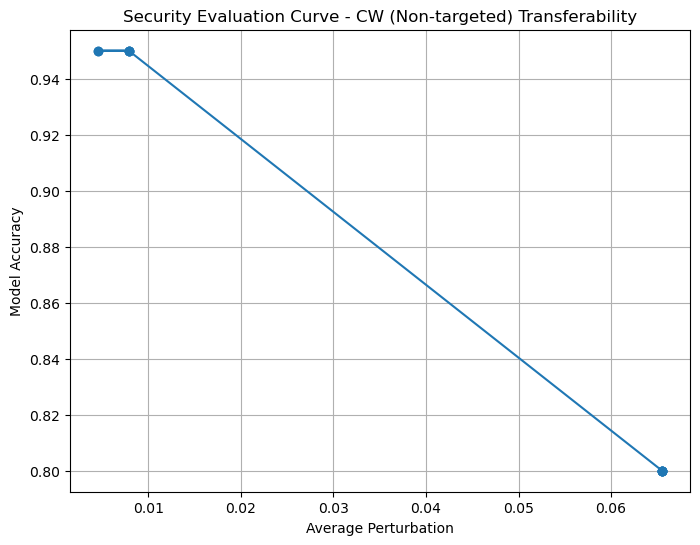
\includegraphics[width=0.7\textwidth]{images/cwtras3.png}
          \caption{Security Evaluation Curve - CW L$\infty$ (Non-targeted) Transferability}
          \label{fig:cw_transfer1}
        \end{figure}
        
        \begin{figure}[H]
          \centering
          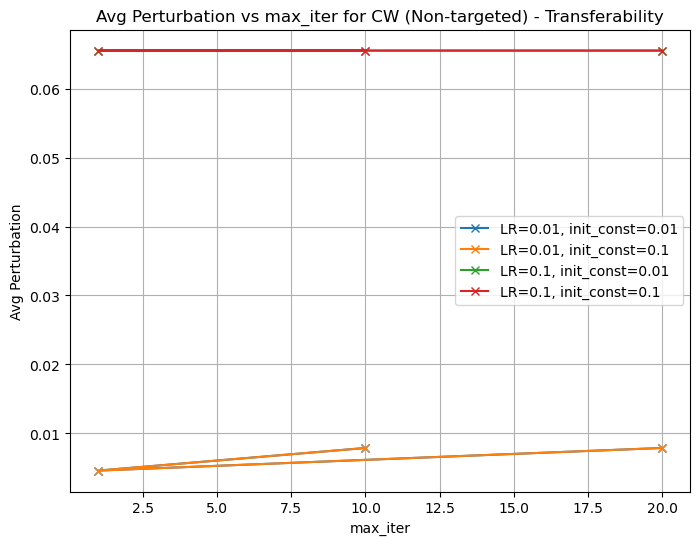
\includegraphics[width=0.7\textwidth]{images/cwtras2.png}
          \caption{Avg Perturbation vs \texttt{max\_iter} per CW L$\infty$ (Non-targeted)}
          \label{fig:cw_transfer2}
        \end{figure}
        
        \begin{figure}[H]
          \centering
          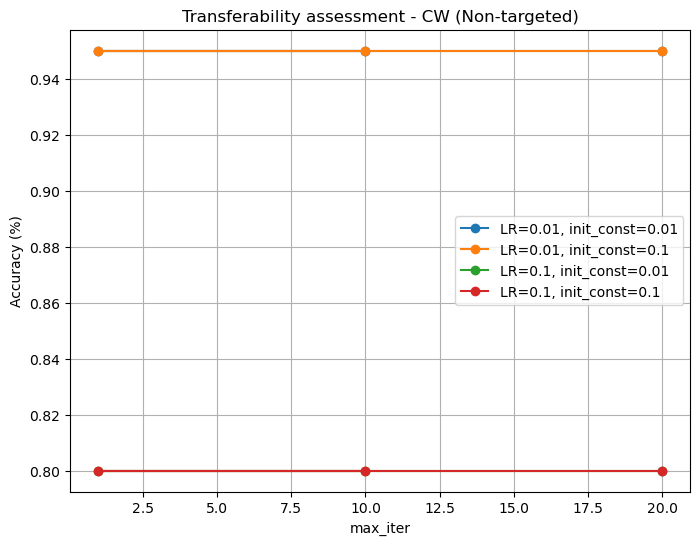
\includegraphics[width=0.7\textwidth]{images/cwtras1.png}
          \caption{Transferability assessment - CW L$\infty$ (Non-targeted)}
          \label{fig:cw_transfer3}
        \end{figure}

        \subsection{Osservazioni}
            I risultati ottenuti indicano un comportamento fortemente dipendente dal valore del learning rate.
            In particolare:
                \begin{itemize}
                  \item Per \texttt{lr = 0.01}, indipendentemente da \texttt{init\_const} e \texttt{max\_iter}, le perturbazioni risultano modeste ($\sim$0.0046--0.0079) e l’accuratezza di NN2 si mantiene elevata ($\sim$95\%).
                  
                  \item Per \texttt{lr = 0.1}, invece, la perturbazione media raggiunge $\sim$0.0655 con $L\infty \sim 0.0999$, producendo un drastico calo dell’accuratezza di NN2 (fino all’80\%).
                \end{itemize}
            
            \noindent I valori numerici sono riassunti nella tabella seguente:
                \begin{center}
                    \begin{tabular}{cccccc}
                        \toprule
                        \textbf{lr} & \textbf{max\_iter} & \textbf{init\_const} & \textbf{Pert. media} & \textbf{L$\infty$} & \textbf{Accuracy (\%)} \\
                        \midrule
                        0.01 & 1  & 0.01 & 0.0046 & 0.0100 & 95.00 \\
                        0.01 & 1  & 0.1  & 0.0046 & 0.0100 & 95.00 \\
                        0.01 & 10 & 0.01 & 0.0079 & 0.0200 & 95.00 \\
                        0.01 & 10 & 0.1  & 0.0079 & 0.0200 & 95.00 \\
                        0.01 & 20 & 0.01 & 0.0079 & 0.0200 & 95.00 \\
                        0.01 & 20 & 0.1  & 0.0079 & 0.0200 & 95.00 \\
                        0.1  & 1  & 0.01 & 0.0655 & 0.0999 & 80.00 \\
                        0.1  & 1  & 0.1  & 0.0655 & 0.0999 & 80.00 \\
                        0.1  & 10 & 0.01 & 0.0655 & 0.0999 & 80.00 \\
                        0.1  & 10 & 0.1  & 0.0655 & 0.0999 & 80.00 \\
                        0.1  & 20 & 0.01 & 0.0655 & 0.0999 & 80.00 \\
                        0.1  & 20 & 0.1  & 0.0655 & 0.0999 & 80.00 \\
                        \bottomrule
                    \end{tabular}
                \end{center}

        \subsection{Analisi}
            L’attacco CW non-targeted mostra una buona trasferibilità solo in presenza di un tasso di apprendimento elevato (\texttt{lr = 0.1}), che consente di superare una soglia di perturbazione tale da compromettere efficacemente NN2. Al contrario, per \texttt{lr = 0.01}, le perturbazioni restano contenute e altamente specifiche per NN1, riducendo l’efficacia in trasferimento.
            Questi risultati confermano che, sebbene CW sia potente in contesti white-box, la sua efficacia in black-box è fortemente condizionata dai parametri di ottimizzazione. Inoltre, la stabilità delle metriche tra diverse configurazioni di \texttt{init\_const} evidenzia come sia il learning rate a dominare il comportamento del trasferimento in questo scenario.

    \section{Trasferibilità dell'attacco Carlini-Wagner L$2$ (Non-targeted)}
        Per l'esperimento è stato utilizzato l'attacco Carlini-Wagner nella variante $L2$ non-targeted, valutando diverse combinazioni dei parametri: \texttt{learning\_rate} $\in \{0.01, 0.1\}$, \texttt{initial\_const} $\in \{0.01, 0.1\}$ e \texttt{max\_iter} $\in \{1, 10, 20\}$. I risultati sono riportati nei grafici in Figura~\ref{fig:cw_untarg_l2_acc}, \ref{fig:cw_untarg_l2_pert} e \ref{fig:cw_untarg_l2_sec}.
        
        \begin{figure}[H]
            \centering
            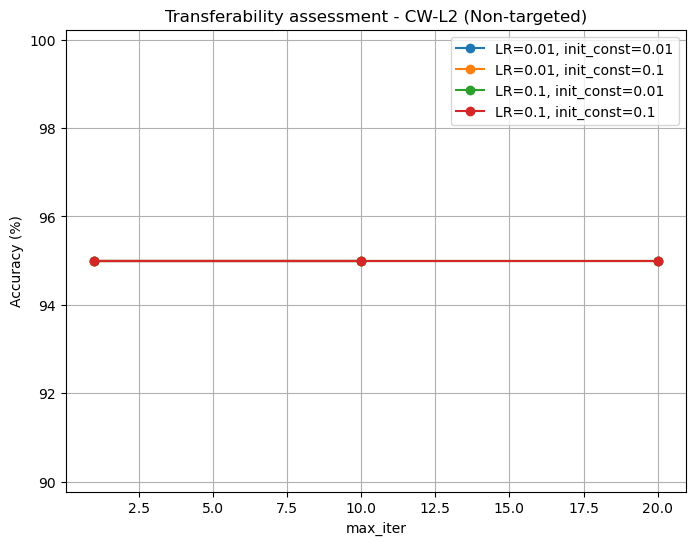
\includegraphics[width=0.6\textwidth]{images/cwtrasuntargl2.png}
            \caption{Accuracy vs max\_iter per Carlini \& Wagner $L2$ (Non-targeted)}
            \label{fig:cw_untarg_l2_acc}
        \end{figure}
        
        \begin{figure}[H]
            \centering
            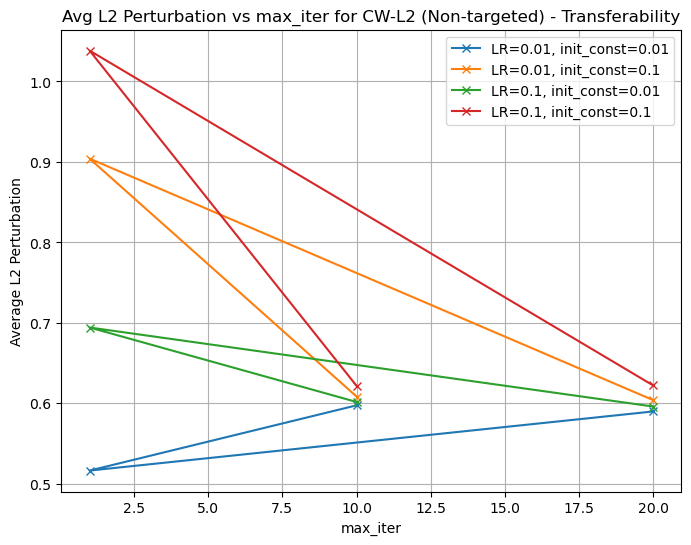
\includegraphics[width=0.6\textwidth]{images/cwtrasuntargl2-1.png}
            \caption{Avg $L^2$ Perturbation vs max\_iter per Carlini \& Wagner $L2$ (Non-targeted)}
            \label{fig:cw_untarg_l2_pert}
        \end{figure}
        
        \begin{figure}[H]
            \centering
            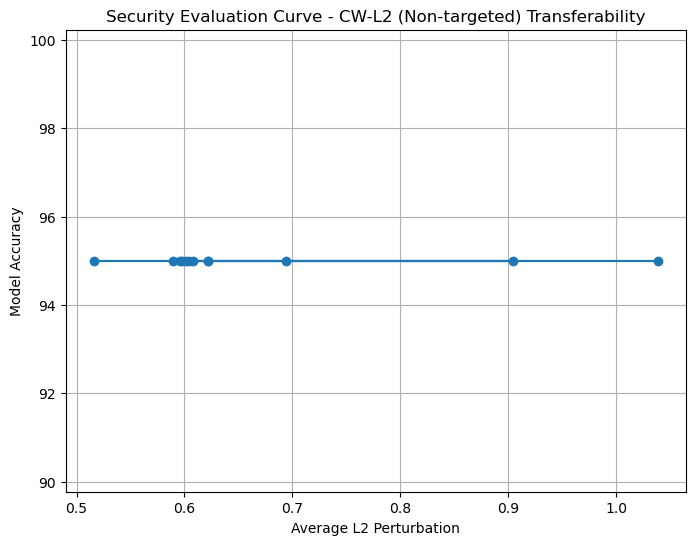
\includegraphics[width=0.6\textwidth]{images/cwtrasuntargl2sec.png}
            \caption{Security Evaluation Curve per Carlini \& Wagner $L2$ (Non-targeted)}
            \label{fig:cw_untarg_l2_sec}
        \end{figure}

        \subsection{Risultati}
            Nel contesto della valutazione di trasferibilità dell'attacco Carlini-Wagner in modalità non-targeted con norma L2, sono stati generati esempi avversari sulla rete sorgente NN1 e successivamente testati sulla rete target NN2. I risultati mostrano che l'attacco \textbf{non è riuscito a trasferirsi in alcuna configurazione}: in tutte le prove, l’accuratezza della rete target NN2 è rimasta invariata al $95\%$, ovvero identica al caso pulito.
            È interessante notare che, nonostante l'assenza di successo nella fase di trasferimento, le perturbazioni medie introdotte non erano trascurabili, con valori di norma $L2$ medi superiori a $0.5$ e massimi fino a $2.77$. Questo indica che il perturbatore ha effettivamente modificato l'immagine in modo misurabile, ma non in maniera sufficiente da compromettere le decisioni del classificatore target.
            Questo comportamento è coerente con quanto osservato in letteratura: gli attacchi Carlini-Wagner sono noti per essere ottimizzati in modo specifico per il modello su cui sono generati, e tendono a generare perturbazioni meno trasferibili rispetto ad altri attacchi come FGSM o BIM. La natura non lineare e altamente mirata dell’ottimizzazione, unita alla ricerca del minimo disturbo visibile, rende l’attacco meno generalizzabile ad architetture diverse.
            In Figura~\ref{fig:cwnt_transf_success},~\ref{fig:cwnt_transf_perturb},~\ref{fig:cwnt_transf_sec} si riportano rispettivamente:
            \begin{itemize}
                \item la curva di accuratezza su NN2 al variare di \texttt{max\_iter} e dei parametri dell’attacco;
                
                \item l’andamento della perturbazione media in norma L2 al crescere delle iterazioni;
                
                \item la Security Evaluation Curve che mostra l’assenza di compromissione anche in presenza di perturbazioni crescenti.
            \end{itemize}
            
            \begin{figure}[H]
                \centering
                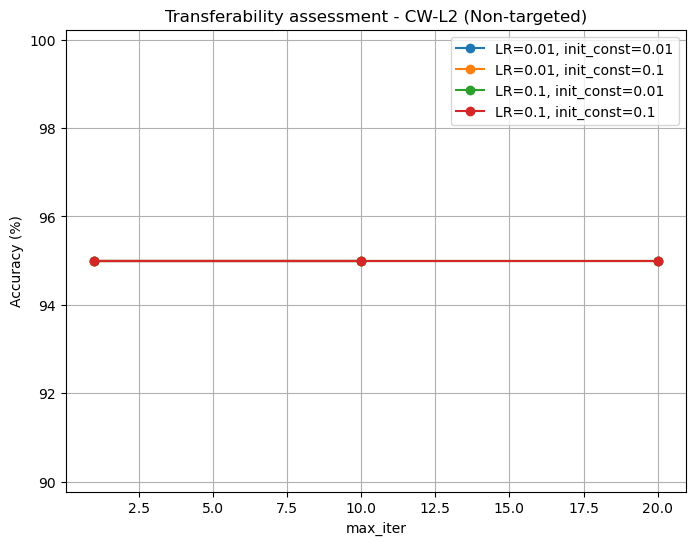
\includegraphics[width=0.55\textwidth]{images/cwtrasuntargl2.png}
                \caption{Transferability assessment - CW-$L2$ (Non-targeted)}
                \label{fig:cwnt_transf_success}
            \end{figure}
            
            \begin{figure}[H]
                \centering
                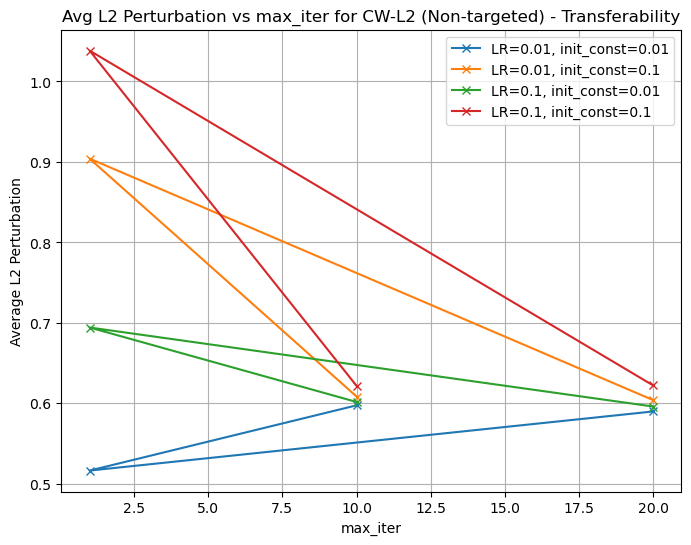
\includegraphics[width=0.55\textwidth]{images/cwtrasuntargl2-1.png}
                \caption{Average L2 Perturbation vs \texttt{max\_iter} - CW-L2 (Non-targeted)}
                \label{fig:cwnt_transf_perturb}
            \end{figure}
            
            \begin{figure}[H]
                \centering
                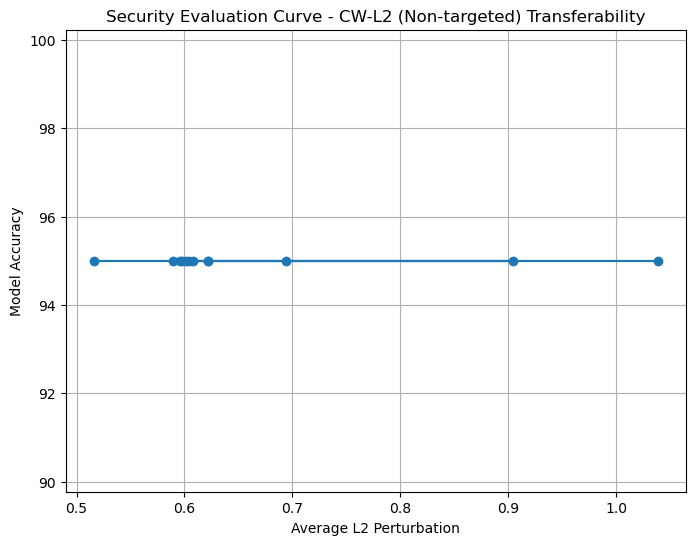
\includegraphics[width=0.55\textwidth]{images/cwtrasuntargl2sec.png}
                \caption{Security Evaluation Curve - CW-L2 (Non-targeted) Transferability}
                \label{fig:cwnt_transf_sec}
            \end{figure}
            
        \subsection{Analisi dei risultati}
            L’analisi complessiva dei risultati suggerisce che, pur essendo il Carlini-Wagner L2 un attacco efficace nel contesto white-box sul modello sorgente (NN1), \textbf{la sua capacità di trasferirsi ad altri modelli risulta estremamente limitata}. Tutte le configurazioni testate non sono riuscite ad alterare significativamente l’accuratezza del modello target (NN2), che è rimasta stabile al $95\%$.
            Questa evidenza conferma quanto riportato in letteratura, dove si sottolinea che gli attacchi CW, ottimizzati attraverso complesse funzioni obiettivo e vincoli di ottimalità su una specifica rete, \textbf{tendono a generare perturbazioni poco generalizzabili}. La mancanza di trasferibilità è particolarmente marcata nei casi in cui il modello target presenta architetture molto diverse rispetto a quello sorgente.
            Un ulteriore elemento di rilievo è che perturbazioni anche relativamente ampie in norma L2 non si sono tradotte in errori di classificazione su NN2. Ciò suggerisce che l’ottimizzazione avviene in una regione del manifold delle immagini molto legata alle specifiche caratteristiche apprese dal modello attaccato, rendendo il trasferimento meno probabile.
            In sintesi, i risultati ottenuti evidenziano come la potenza del Carlini-Wagner L2 sia fortemente legata al contesto white-box e pongono l’attenzione sulla necessità di combinare attacchi o progettare strategie più generalizzabili per analisi di robustezza cross-model.

    \section{Confronto tra gli Attacchi Non-Targeted}
        \begin{itemize}
          \item Gli attacchi iterativi come \textbf{BIM} e \textbf{PGD} ottengono i risultati più incisivi in termini di abbattimento dell’accuratezza su NN2, con valori inferiori al 42\%, a fronte di perturbazioni medie relativamente contenute ($\sim$0.06).
          
          \item L’attacco \textbf{FGSM}, pur essendo il più semplice, mostra un comportamento competitivo, ma richiede un livello di distorsione maggiore per ottenere un degrado simile.
          
          \item \textbf{DeepFool} si conferma altamente efficace in white-box, ma scarsamente trasferibile, con una perturbazione quasi nulla e una accuratezza residuale molto elevata su NN2 ($\sim$96\%).
          
          \item \textbf{Carlini-Wagner} mostra una trasferibilità significativa solo in presenza di learning rate elevati, risultando meno pericoloso in modalità black-box rispetto a PGD e BIM.
        \end{itemize}

        \noindent Nel complesso, gli attacchi iterativi proiettati (PGD e BIM) rappresentano la minaccia più rilevante in scenari black-box, grazie alla loro capacità di generare perturbazioni robuste e generalizzabili. Gli attacchi ottimizzati come CW sono invece più sensibili ai parametri e meno efficaci in trasferimento se non correttamente calibrati.

    \section{Trasferibilità dell'attacco FGSM Targeted}
        L'attacco \textbf{FGSM targeted}, applicato sulla rete NN1, è stato testato per verificarne la \textit{trasferibilità} verso il classificatore NN2 (basato su ResNet50). Lo scopo è determinare se le perturbazioni, progettate per forzare una classificazione errata verso una \textit{classe bersaglio} su NN1, riescano a generare lo stesso effetto anche su un modello con architettura differente.
        Il grafico in Figura~\ref{fig:fgsm_targeted_transfer} mostra l'andamento della \textit{Targeted Attack Success Rate} rispetto alla \textit{perturbazione media introdotta} nei campioni.

        \begin{figure}[H]
          \centering
          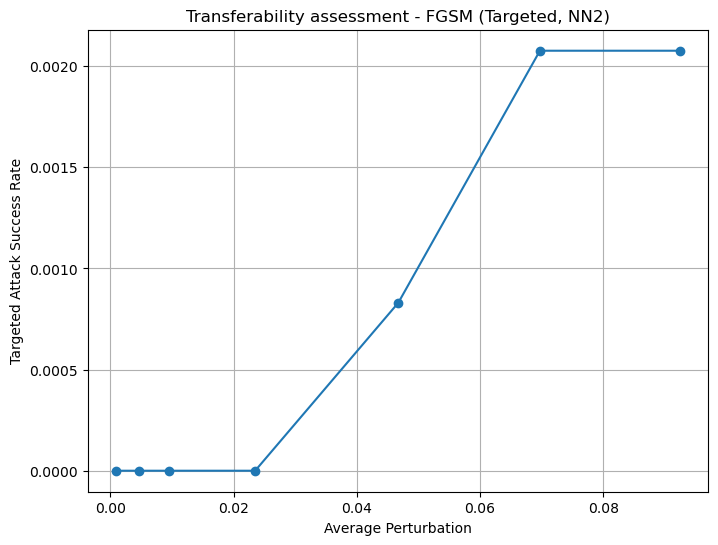
\includegraphics[width=0.65\textwidth]{images/fgsm_targeted_transferability.png}
          \caption{Transferability assessment - FGSM (Targeted, NN2).}
          \label{fig:fgsm_targeted_transfer}
        \end{figure}

        \subsection{Osservazioni}
            I risultati numerici indicano un tasso di successo nullo per valori di perturbazione media inferiori a $0.04$ e solo un modesto incremento nei casi più estremi:
                \begin{center}
                    \begin{tabular}{ccc}
                        \toprule
                        \textbf{Perturbazione media} & \textbf{L$_\infty$} & \textbf{Tasso di successo (\%)} \\
                        \midrule
                        0.0009 & 0.0010 & 0.00 \\
                        0.0047 & 0.0050 & 0.00 \\
                        0.0094 & 0.0100 & 0.00 \\
                        0.0235 & 0.0250 & 0.00 \\
                        0.0467 & 0.0500 & 0.08 \\
                        0.0697 & 0.0750 & 0.21 \\
                        0.0924 & 0.1000 & 0.21 \\
                        \bottomrule
                    \end{tabular}
                \end{center}

        \subsection{Analisi}
            L’attacco FGSM targeted si è dimostrato scarsamente trasferibile su NN2. Anche per livelli elevati di distorsione (L$\infty$ fino a 0.1), il tasso di successo rimane trascurabile (al massimo $\sim0.2\%$), a fronte di un successo superiore al 14\% osservato su NN1. Questo risultato conferma che l’attacco FGSM, basato su una singola iterazione lungo la direzione del gradiente, tende a produrre perturbazioni altamente specifiche per l’architettura bersaglio originale.
            In letteratura, è noto che gli attacchi \textit{targeted} sono generalmente meno trasferibili rispetto ai \textit{non-targeted}, a causa della maggiore precisione richiesta nel forzare la predizione verso una classe scelta dall’attaccante. Come evidenziato in studi come \textit{Liu et al., 2017} e \textit{Goodfellow et al., 2015}, la trasferibilità tende a decrescere all’aumentare della specificità dell’obiettivo dell’attacco.

    \section{Trasferibilità dell'attacco BIM Targeted}
        In questo esperimento è stata analizzata la trasferibilità dell’attacco \textbf{Basic Iterative Method (BIM)}, in modalità \textit{targeted}, verso il classificatore NN2 (ResNet50). L’obiettivo è valutare se le perturbazioni costruite per forzare la predizione di NN1 verso una specifica classe siano efficaci anche su una rete architetturalmente distinta.
        Il grafico in Figura~\ref{fig:bim_targeted_transfer} rappresenta l’evoluzione del \textit{Targeted Attack Success Rate} in funzione della \textit{perturbazione media}, variando i parametri \texttt{max\_iter} e $\epsilon$.

        \begin{figure}[H]s
          \centering
          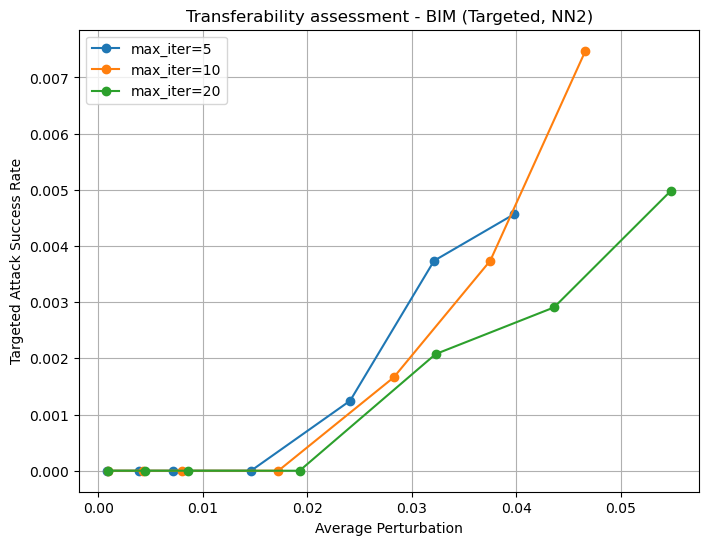
\includegraphics[width=0.7\textwidth]{images/bim_targeted_transferability.png}
          \caption{Transferability assessment - BIM (Targeted, NN2).}
          \label{fig:bim_targeted_transfer}
        \end{figure}

        \subsection{Risultati}
            I risultati mostrano che l'attacco BIM targeted mantiene una scarsa capacità di trasferirsi a NN2. Per perturbazioni deboli (L$\infty \leq 0.025$), il tasso di successo è nullo indipendentemente dal numero di iterazioni. Solo a partire da $\epsilon = 0.05$, si osserva un leggero incremento:
            
            \begin{itemize}
              \item Per $\epsilon = 0.05$, \texttt{max\_iter} = 5, il tasso di successo è pari allo 0.12\%.
              \item Aumentando a \texttt{max\_iter} = 10 e 20, si ottengono rispettivamente successi dello 0.17\% e 0.21\%.
              \item Con $\epsilon = 0.1$, si raggiungono i valori massimi osservati: fino allo 0.75\% con \texttt{max\_iter} = 10.
            \end{itemize}

            \noindent Nonostante la maggiore potenza dell’attacco iterativo rispetto al FGSM, i risultati confermano che la \textbf{trasferibilità degli attacchi targeted è intrinsecamente limitata}, in particolare quando si considerano modelli profondamente diversi (NN1 vs NN2).

        \subsection{Discussione}
            BIM, essendo una versione iterativa di FGSM, produce perturbazioni localmente più efficaci nel dominio del modello bersaglio. Tuttavia, queste perturbazioni sembrano ottimizzate in modo troppo specifico per l’architettura NN1 e raramente riescono a guidare NN2 verso la classe bersaglio desiderata.
            Come evidenziato in letteratura (\textit{Liu et al., 2017}), gli attacchi \textit{targeted} richiedono una precisa manipolazione della distribuzione delle attivazioni intermedie, il che riduce la probabilità di successo su modelli non identici. Inoltre, la strategia di trasferire classi bersaglio tramite mappatura ciclica potrebbe accentuare questa difficoltà.

    \section{Trasferibilità dell'attacco PGD Targeted}
        L’attacco \textbf{Projected Gradient Descent (PGD)} consente di esplorare con maggiore efficacia il dominio locale di input, massimizzando la probabilità di ingannare il classificatore. In questa sezione ne analizziamo la trasferibilità, in modalità \textit{targeted}, dalla rete NN1 alla rete ResNet50 (NN2).
        Il grafico di Figura~\ref{fig:pgd_targeted_transfer} mostra il tasso di successo dell’attacco in funzione della perturbazione media, al variare del parametro \texttt{max\_iter}.
        
        \begin{figure}[H]
          \centering
          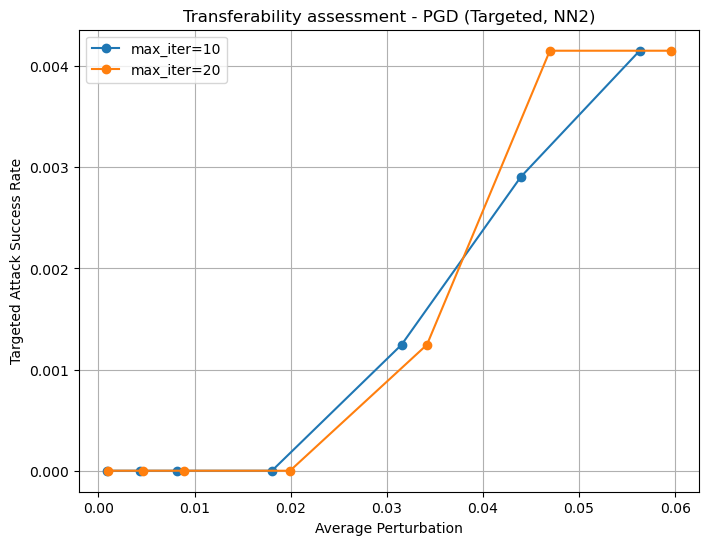
\includegraphics[width=0.7\textwidth]{images/pgd_targeted_transferability.png}
          \caption{Transferability assessment - PGD (Targeted, NN2).}
          \label{fig:pgd_targeted_transfer}
        \end{figure}

        \subsection{Risultati}
            I risultati indicano che la probabilità di successo dell’attacco PGD targeted su NN2 è estremamente bassa. Nella maggior parte dei casi, il tasso di successo rimane nullo fino a perturbazioni superiori a 0.03. Alcune osservazioni chiave includono:
            
            \begin{itemize}
              \item Per $\epsilon \leq 0.025$, il \textit{Targeted Success Rate} è sempre 0\%.
              \item A partire da $\epsilon = 0.05$, si ottiene un successo marginale dello 0.12\%.
              \item Con $\epsilon = 0.075$ e \texttt{max\_iter} = 20, il successo sale fino allo 0.42\%.
              \item Aumentare ulteriormente \texttt{max\_iter} non produce miglioramenti significativi oltre tale soglia.
            \end{itemize}
            
        \subsection{Discussione}
            Sebbene PGD sia riconosciuto in letteratura (\textit{Madry et al., 2018}) come uno degli attacchi più robusti in scenari \textit{white-box}, i risultati ottenuti suggeriscono che in modalità \textit{targeted} esso non riesca a trasferirsi efficacemente a modelli differenti.
            Il motivo risiede nella natura \textit{direzionale} dell’attacco. PGD, infatti, cerca specificamente di forzare il modello a classificare l'immagine come una classe target, ottimizzando una traiettoria molto precisa nello spazio delle immagini. Questa traiettoria, sebbene efficace su NN1, perde coerenza semantica quando valutata su NN2.
            Anche la componente stocastica del PGD (un solo \texttt{random\_init} in questo caso) potrebbe non essere sufficiente a generare perturbazioni generalizzabili ad altri modelli. Un incremento del numero di inizializzazioni casuali potrebbe migliorare leggermente la trasferibilità, ma a scapito del tempo computazionale.

        \subsection{Conclusione}
            La trasferibilità del PGD targeted su NN2 risulta limitata. Anche con perturbazioni consistenti ($\epsilon = 0.1$), il tasso di successo non supera lo 0.42\%. Questo comportamento conferma quanto osservato per gli altri attacchi targeted, l’ottimizzazione verso una classe specifica tende a produrre perturbazioni fortemente legate alla rete su cui vengono generate, rendendo difficile la generalizzazione cross-architettura.

    \section{Trasferibilità dell'attacco Targeted Carlini-Wagner L$\infty$ }
        L'attacco \textit{Carlini-Wagner} con norma L$\infty$ è stato eseguito in modalità \textit{targeted} sulla rete NN1 e successivamente è stata valutata la sua trasferibilità su NN2. L’obiettivo era verificare se gli esempi avversari potessero forzare NN2 a classificare le immagini secondo le etichette target predefinite, ossia la classe successiva modulo $N$.

        \subsection{Parametri dell'esperimento}
            L'attacco è stato testato su un sottoinsieme di 20 immagini del test set, selezionate casualmente.
            I parametri esplorati includono:
                \begin{itemize}
                  \item \textbf{Learning rate}: \texttt{0.01}, \texttt{0.1}
                  \item \textbf{Max iterazioni}: \texttt{1}, \texttt{10}, \texttt{20}
                  \item \textbf{Initial constant}: \texttt{0.01}, \texttt{0.1}
                \end{itemize}

        \subsection{Risultati}
            I risultati mostrano che, nonostante la variazione dei parametri, \textbf{il tasso di successo dell'attacco targeted trasferito è rimasto costantemente pari a 0\%} per tutte le combinazioni. Questo indica che nessun esempio avversario ha indotto NN2 a classificare correttamente secondo la classe target desiderata.
            In particolare, anche nei casi in cui la perturbazione media era relativamente elevata (ad esempio con \texttt{LR=0.1}, \texttt{max\_iter=1}), la rete NN2 ha sempre fallito nel classificare le immagini nella classe target. Le curve riportate confermano questi risultati:
                \begin{itemize}
                  \item \textbf{Figura \ref{fig:cwlinf-transfer-accuracy}} mostra il \textit{Targeted Success Rate} rispetto a \texttt{max\_iter}, evidenziando valori nulli indipendentemente dai parametri.
                  
                  \item \textbf{Figura \ref{fig:cwlinf-transfer-perturb}} rappresenta la perturbazione media introdotta in funzione di \texttt{max\_iter}. Si osservano picchi iniziali che si annullano completamente per iterazioni più elevate.
                  
                  \item \textbf{Figura \ref{fig:cwlinf-transfer-sec}} è la \textit{Security Evaluation Curve}, che evidenzia come l'incremento della perturbazione non si traduca in alcun successo dell’attacco.
                \end{itemize}
            
            \begin{figure}[H]
              \centering
              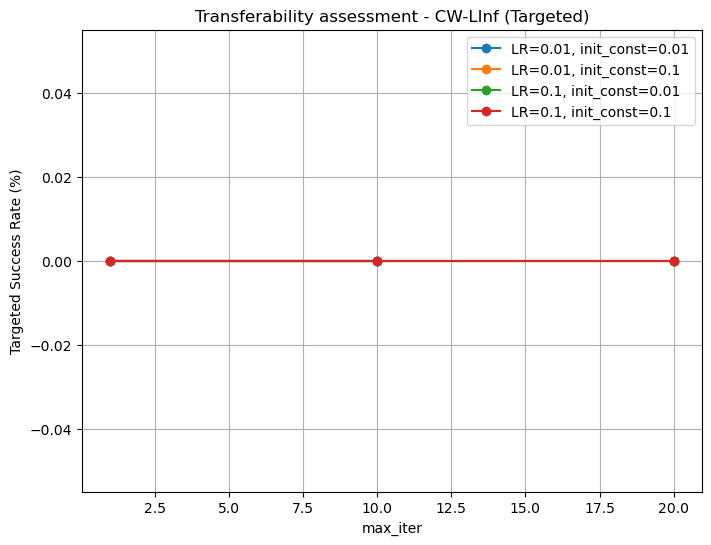
\includegraphics[width=0.65\textwidth]{images/cwlinf_transfer_accuracy.png}
              \caption{Transferability assessment - CW-L$\infty$ (Targeted)}
              \label{fig:cwlinf-transfer-accuracy}
            \end{figure}
            
            \begin{figure}[H]
              \centering
              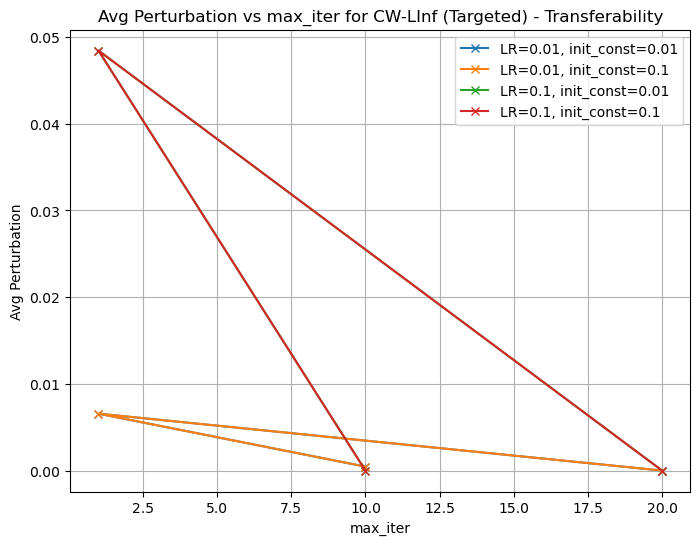
\includegraphics[width=0.65\textwidth]{images/cwlinf_transfer_perturb.png}
              \caption{Avg Perturbation vs max\_iter - CW-L$\infty$ (Targeted) - Transferability}
              \label{fig:cwlinf-transfer-perturb}
            \end{figure}
            
            \begin{figure}[H]
              \centering
              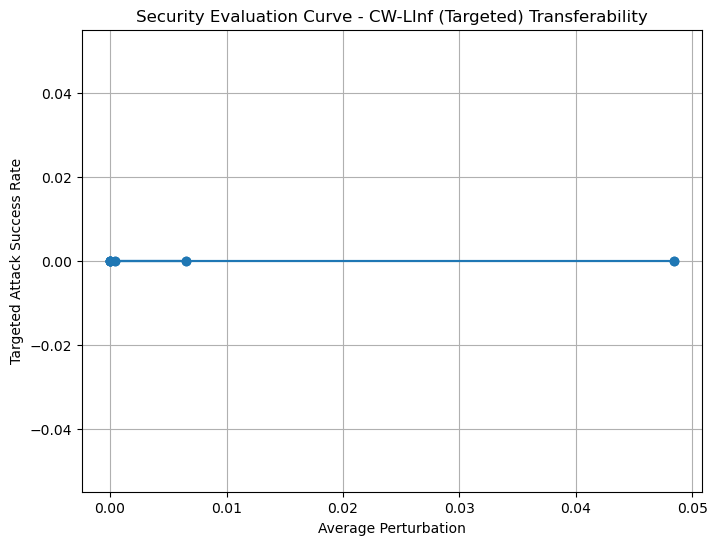
\includegraphics[width=0.65\textwidth]{images/cwlinf_transfer_sec_eval.png}
              \caption{Security Evaluation Curve - CW-L$\infty$ (Targeted) - Transferability}
              \label{fig:cwlinf-transfer-sec}
            \end{figure}

        \subsection{Discussione}
            Il comportamento osservato è coerente con quanto riportato in letteratura: gli attacchi Carlini-Wagner, pur essendo potenti sul modello sorgente, tendono a non trasferirsi efficacemente. Questo accade perché il metodo CW ottimizza perturbazioni molto specifiche rispetto alla funzione obiettivo e ai gradienti del modello attaccato, producendo perturbazioni difficili da generalizzare su modelli con architettura diversa.
            Inoltre, nella modalità targeted, la condizione è ancora più restrittiva, in quanto non è sufficiente ingannare il classificatore, ma bisogna forzarlo a produrre una specifica predizione. Ciò rende la trasferibilità ancora meno probabile.

    \section{Trasferibilità dell'attacco Targeted Carlini-Wagner L2}
        In questa sezione analizziamo la capacità di trasferimento verso NN2 degli adversarial samples generati tramite l’attacco \textbf{Carlini \& Wagner con norma L2} in modalità \textit{targeted}. A differenza della versione \textit{error-generic}, l’obiettivo di questo attacco è forzare il classificatore ad assegnare un’etichetta specifica (target) a ciascuna immagine, rendendo l’analisi della trasferibilità particolarmente interessante in un contesto black-box.
        I risultati sono riportati nei seguenti grafici.
        
        \begin{figure}[H]
          \centering
          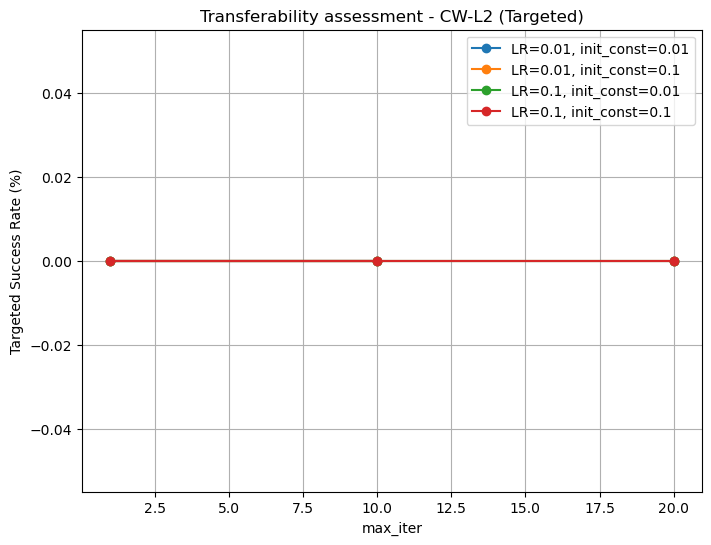
\includegraphics[width=0.75\textwidth]{images/cwtrastargl2.png}
          \caption{Transferability assessment - CW-L2 (Targeted)}
        \end{figure}
        
        \begin{figure}[H]
          \centering
          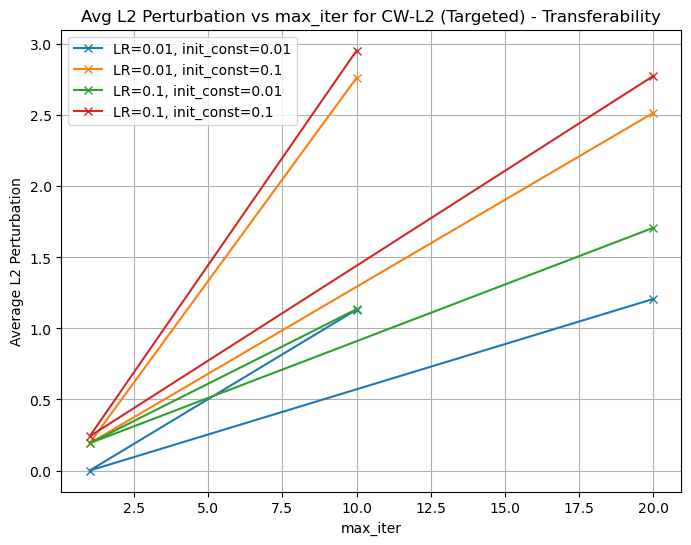
\includegraphics[width=0.75\textwidth]{images/cwtrastargl2-1.png}
          \caption{Avg L2 Perturbation vs max\_iter for CW-L2 (Targeted) - Transferability}
        \end{figure}
        
        \begin{figure}[H]
          \centering
          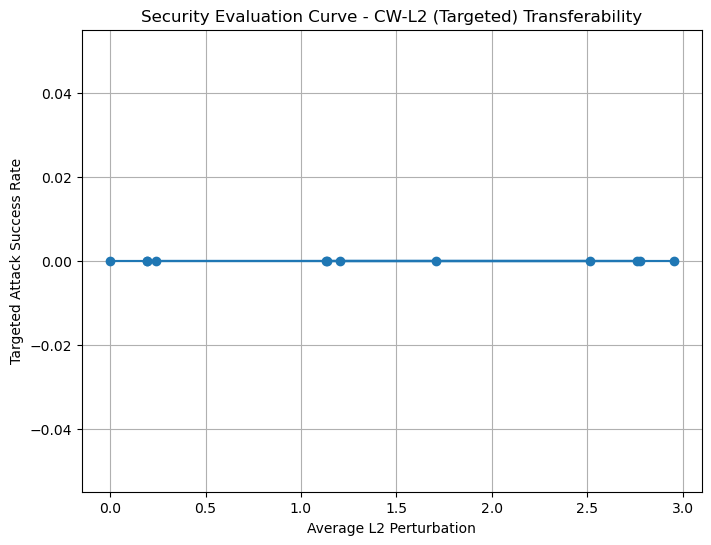
\includegraphics[width=0.75\textwidth]{images/cwtrastargl2sec.png}
          \caption{Security Evaluation Curve - CW-L2 (Targeted) Transferability}
        \end{figure}

        \subsection{Analisi dei risultati}
            Come evidenziato dai grafici, nonostante la presenza di perturbazioni anche significative (con valori medi di norma L2 superiori a 2.5 per alcune configurazioni), la \textbf{success rate} dell’attacco su NN2 è risultata nulla in tutti i casi analizzati. Nemmeno per valori elevati di \texttt{initial\_const} e \texttt{max\_iter} è stato ottenuto un singolo successo nell’indurre NN2 a classificare l’immagine nella classe target desiderata.
            Questo risultato conferma la scarsa trasferibilità degli attacchi Carlini-Wagner L2 in modalità targeted, già osservata in letteratura. Tali attacchi tendono infatti a produrre perturbazioni molto precise e specifiche per l'architettura, difficilmente generalizzabili a modelli differenti, specialmente quando la struttura (NN1 vs NN2) cambia significativamente.
            L’andamento della curva di sicurezza mostra inoltre una decisa separazione tra l’aumento della perturbazione e il mancato guadagno in termini di successo, suggerendo un’inefficacia strutturale nella generalizzazione dell’attacco.

    \section{Confronto sulla Trasferibilità degli Attacchi Targeted}
        Come già detto in precedenza, la misura utilizzata per quantificare l'efficacia del trasferimento è la \textit{Targeted Attack Success Rate}, ovvero la percentuale di campioni per cui la rete target ha predetto correttamente la classe obiettivo imposta dall'attacco.
        I risultati confermano un comportamento coerente con quanto noto in letteratura:
            \begin{itemize}
                \item \textbf{FGSM}: presenta un successo di trasferibilità molto basso (max $\approx 0.21\%$), anche per valori elevati di perturbazione. Questo è coerente con la sua natura one-step e la direzionalità debole della perturbazione.
                
                \item \textbf{BIM} e \textbf{PGD}: migliorano leggermente rispetto a FGSM (fino a circa $0.75\%$), ma restano comunque scarsamente efficaci in ottica targeted transfer. Entrambi sono gradient-based iterativi, ma risultano sensibili alla specificità del modello.
                
                \item \textbf{CW (L$\infty$ e L$2$)}: completamente inefficace nella modalità targeted. Nessuna configurazione di iperparametri ha portato a un singolo caso di successo, a testimonianza della forte specializzazione dell'attacco.
            \end{itemize}

        \noindent Riassumendo, tutti gli attacchi targeted presentano \textbf{trasferibilità estremamente limitata}, con tassi di successo spesso inferiori all’1\%. Questo comportamento è dovuto al fatto che le perturbazioni targeted tendono ad essere molto precise e \textit{model-specific}, ottimizzate per portare la rete ad una classe ben definita, e quindi scarsamente generalizzabili su modelli differenti.